\documentclass[11pt,a4paper]{article}
\usepackage{bbm,amsthm,amsfonts,amssymb,amsmath,latexsym,epic,eepic}
\usepackage{marvosym,graphicx,fancyhdr,bbm}
\usepackage{graphicx}
\usepackage{color}
\usepackage[rflt]{floatflt}
\usepackage{colortbl}
\usepackage{subcaption}
\usepackage[vlined, ruled, boxed]{algorithm2e}
\definecolor{Grey}{rgb}{0.5,0.5,0.5}
\definecolor{Red}{rgb}{1.0,0.0,0.0}

\usepackage{typearea}
\areaset{156mm}{235mm}
%\setlength{\parskip}{5pt plus 2pt minus 1pt}
\setlength{\parindent}{0pt}

% use \M for matrices and \V for vectors in math mode
\newcommand{\M}[1]{\mathbf{#1}}
\newcommand{\V}[1]{\mathbf{#1}}
\newcommand{\norm}[1]{\left | \left | #1 \right | \right |}
\newcommand{\RR}{\mathbbm{R}}        % set of real numbers


\renewcommand\floatpagefraction{0.8}
\renewcommand\topfraction{1}
\renewcommand\bottomfraction{0.9}
\renewcommand\textfraction{0.0}
%\def\dbltopfraction{1.0}
%\def\bottomfraction{1.0}
%\def\dblfloatpagefraction{0.8}


\makeatletter
\renewenvironment{thebibliography}[1]
     {\section*{\refname}%
      \@mkboth{\MakeUppercase\refname}{\MakeUppercase\refname}%
	 \parsep0mm
	 \itemsep0mm
	 %\labelsep0mm
	 %\itemindent0mm
      \list{\@biblabel{\@arabic\c@enumiv}}%
           {\settowidth\labelwidth{\@biblabel{#1}}%
            \leftmargin\labelwidth
            \advance\leftmargin\labelsep
            \@openbib@code
            \usecounter{enumiv}%
            \let\p@enumiv\@empty
            \renewcommand\theenumiv{\@arabic\c@enumiv}}%
      \sloppy
      \clubpenalty4000
      \@clubpenalty \clubpenalty
      \widowpenalty4000%
      \sfcode`\.\@m}
     {\def\@noitemerr
       {\@latex@warning{Empty `thebibliography' environment}}%
      \endlist}
\renewcommand\newblock{\hskip .11em\@plus.33em\@minus.07em}
\let\@openbib@code\@empty
\makeatother



\begin{document}\sloppy

\title{\Large\bf Vergleich der Pfadverfolgung mit Odometrie und AMCL \footnotetext{Diese Arbeit ist Bestandteil des Praktikums zur Mess- und Regelungstechnik}}

\author{Kai Hofmann und Barbara Fischbach\\
  Robotik und Telematik \\
  Universit\"at W\"urzburg\\
  Am Hubland, D-97074 W\"urzburg\\
{\small \texttt{barbara.fischbach@uni-wuerzburg.de}}\\
{\small \texttt{kai.hofmann@uni-wuerzburg.de}}}

\date{}



\maketitle


\newpage

\twocolumn

\section*{Abstract}

\addcontentsline{toc}{section}{Abstract}

\textbf{Die autononome Fortbewegung von Fahrzeugen spielt heutzutage eine immer gr\"o\ss{}ere Rolle. Dazu werden verschiedene Algorithmen, zur Lokalisierung, Kartierung und Pfadverfolgung ben\"otigt. Diese werden auf einer realen Roboter-Platform implementiert und getestet.}

Nicht nur im Weltall, wo wir unbedingt darauf angewiesen sind, dass Systeme autonom funktionieren, sondern auch auf der Erde, um Systeme sicherer und bequemer f\"ur den Benutzer zu machen. 


\section{Einleitung}
	Selbstfahrende Fahrzeuge sind ein gro{\ss}es Thema der Zukunft. Damit diese zuverlässig und sicher fahren können braucht es gute Algorithmen in verschiedenen Bereichen. Wie gut bestehende Ans\"atze funktionieren und wo deren Schw\"achen sind wird in diesem Paper anhand einer simplen Roboter-Plattform mit Laserscanner untersucht. 

	Zur Lokalisierung in einer zuvor kartierten Umgebung kann der s \textit{Adaptive Monte Carlo Localization}-Algorithmus von XYZ im Paper zx vorgestellt verwendet werden. 
	
	Die daf\"ur ben\"otigte Karte kann mit dem \textit{SLAM-Gmapping}-Algorithmus generiert werden. Dieser löst dass Problem der gleichzeitigen Lokalisation und Kartierung durch die Nutzung des Laserscanners schon bei der Lokalisation und nicht erst bei der Kartiertung.
	
	Mit einer guten Lokalisation ist es m\"oglich einem Pfad zu folgen. Dafür hat Giovanni Indiveri den XYZ Algorithmus im Paper zxy beschrieben entwickelt. 


	Die drei Algorithmen werden im Abschnitt 2 genauer erkl\"art. Im Abschnitt 3 folgt eine kurze Beschreibung unserer Testplattform und dem \textit{Robot Operating System}. Die Test-Ergebnisse werden im Abschnitt 4 vorgestellt und disskutiert.
  
\newpage

\section{Algorithmen}

\subsection{Lokalisation}
\subsubsection{Odometrie}
{
	Die Odometrie beruht auf einer relativen Positionsbestimmung, dabei wird aus der vorher bekannten Position des Roboters und der zur\"uckgelegten Weg-strecke die neue Position berechnet. Die vermutliche Wegstrecke wird über die Steuerungsbefehle und ein Modell des Roboters berechnet. Da es kein weiteres Feed back über die Position gibt ist das eine "Open loop". 
}
\subsubsection{Adaptive Monte Carlo Localization} \cite{mclWiki}
{
	Im folgenden als AMCL abgek\"urzt, ist ein Algorithmus der mit Hilfe eines Partikelfilters die Position eines Roboters bestimmt. Dazu wird eine Karte der Umgebung ben\"otigt. Da die Pose zu Beginn nicht bekannt ist, stellt der Roboter Hypothesen dar\"uber auf der Karte an, verteilt also die Partikel \"uber den Zustandsraum. Die anf\"angliche Verteilung auf der Karte kann verschieden sein. Es ist zum Beispiel m\"oglich diese  gleichm\"a{\ss}ig über die ganze Karte zu verteilen. 
	Bei der von den Autoren verwendeten Implementation von AMCL ist sie Gau{\ss}-verteilt um eine gegebene anf\"angliche, gegebene Pose. Ist der Roboter tatsälich an einem anderen Ort, so hat er keine Chance sich zu lokalisieren. 

\begin{figure}[h]
	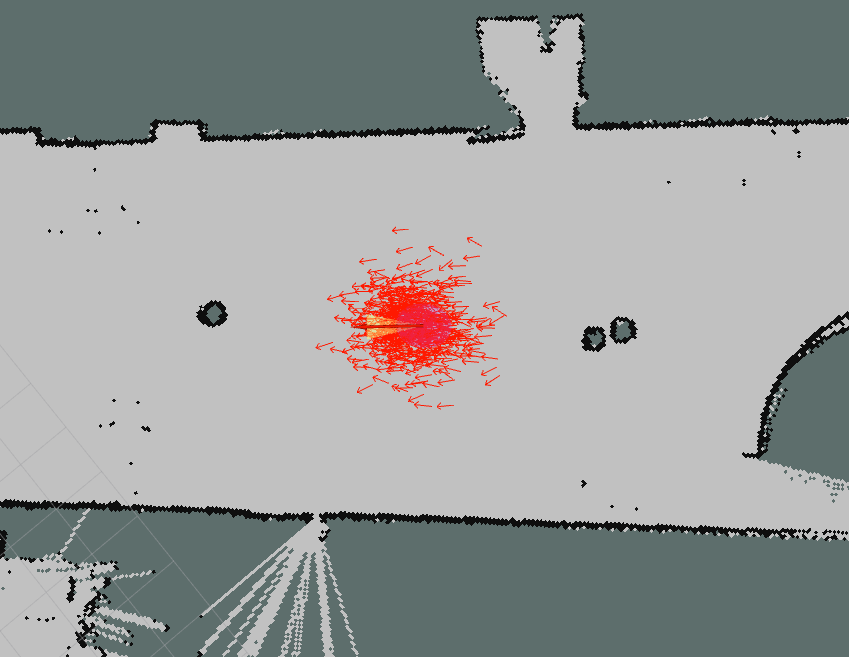
\includegraphics[width=\linewidth]{pictures/initial_distribution.jpg}
	\caption{Partikelverteilung in Anfangspose}
\end{figure}
	
	Die Hypothesen kann man sich als virtuelle Roboter auf der Karte vorstellen. F\"ahrt der reale Roboter, so fahren auch die virtuellen Roboter, mit den gleichen Steuerungsbefehlen. Die realen Sensorwerte werden mit denen der virtuellen Robotern verglichen. Die virtuellen Roboter gewinnen ihre Sensormesswerte durch die Karte. Als reale Sensormesswerte werden die Messungen des Laserscanners verwendet.
	
	Je unstimmiger die Daten des virtuellen Roboters sind, desto unwahrscheinlicher ist die Hypothese dass der reale sich dort befindet. Daher werden jene Partikel gel\"oscht. Im Bereich der wahrscheinlichen Hypothesen, werden neue Partikel/Hypothesen erzeugt.
	
\begin{figure}[h]
	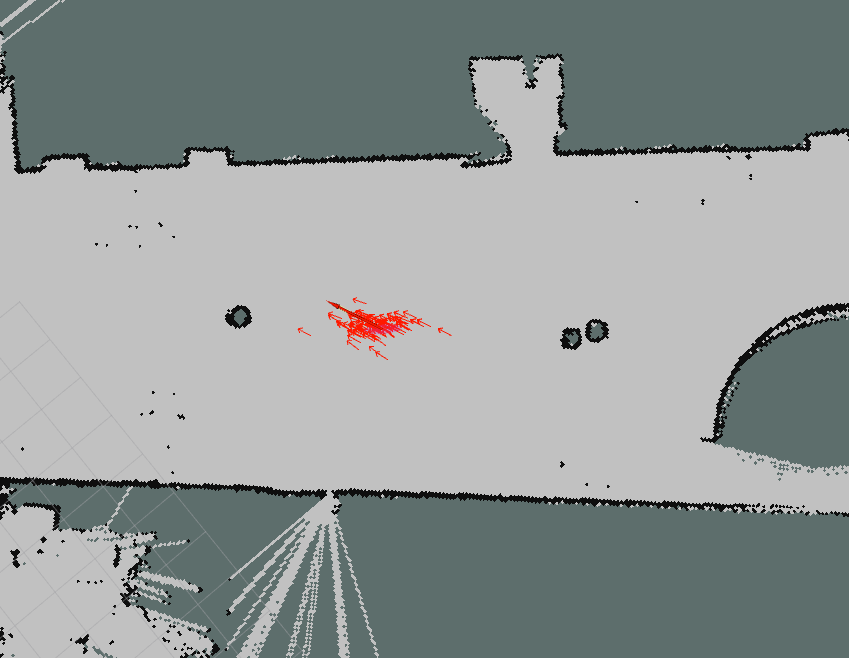
\includegraphics[width=\linewidth]{pictures/drive_little.jpg}
	\caption{Partikelverteilung nach kurzer Neuorientrierung durch Bewegung. Man erkennt die Partikel sind konzentrierter}
\end{figure}
		
	Der virtuelle Roboter  mit besten den \"Ubereinstimmungen, ist die beste Estimation der Pose.
	Je n\"aher die wahrscheinliche Hypothesen bei einander liegen, desto sicherer ist der Roboter sich seiner Pose. Raus finden was adaptive bedeutet bei AMCL.		
}
\newpage
\subsection{Kartierung mit gmapping  \cite{gmapping}}
{
	Die Lokalisation eines Roboters ben\"otigt eine Karte. Eine unbekannte Umgebung wird dabei mit den Daten eines Laserscanners und den aktuellen Posedaten erfasst und von dem Algorithmus GMapping verarbeitet.
	Die Herausforderung liegt dabei in der gleichzeitigen Lokalisierung und Kartierung, dem \textit{simultaneous localization and mapping} Problem kurz SLAM. Denn beide bedingen sich gegenseitig. Um zum Beispiel zwei Laserscans zu einer Karte zusammenzuf\"ugen, m\"ussen die relativen Posen der Aufnahmen bekannt sein. Also ein Lokalisierungsproblem. Und um sich mit dem Laserscanner zu lokalisieren, ben\"otigt man wiederum Kartendaten. \\

	Die Idee des  \textit{Grid}Mappings ist, die ungenauen Sensordaten einer Umgebung, auf einer 2D-Karte in bin\"aren Zufallsvariablen darzustellen. Dabei wird die Karte in Gitter unterteilt, in dem jedes Quadrat mit einer Wahrscheinlichkeit aussagt, ob es belegt ist oder nicht. Die Variablen stellen also Objekte in der Umgebung dar. Algorithmen, wie AMCL, werten die Zufallsvariablen aus. 
	\\ 
	\\

\subsection{Pfadverfolgung mit Giovanni-Controller}


\begin{figure}[h]
	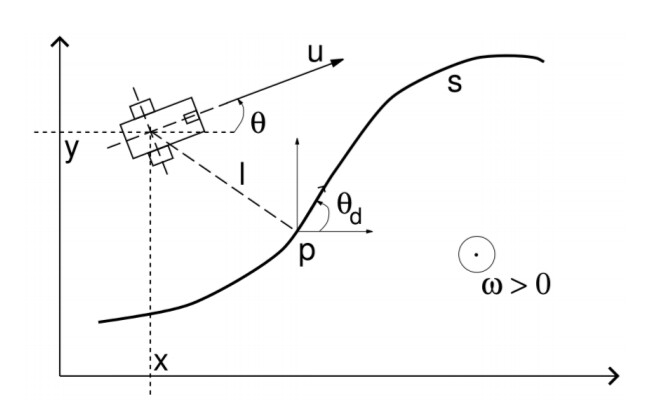
\includegraphics[width=\linewidth]{pictures/Pfadverfolgung.JPG}
	\caption{Modell der Pfadverfolgung}
\end{figure}

	Der nicht-lineare Regler des Giovanni Indiveri und der Maria L. Corradini\cite{Giovanni} wird zur Pfadverfolgung verwendet. Er basiert auf der Arbeit von Canudas de Wit et al. \cite{Canudas} und ist um eine Funktion erweitert, die den  minimalen Wendekreis, wie auch die maximale Geschwindigkeit des Roboters ber\"ucksichtigt. Die Implementierung garantiert nach Lyapunov, f\"ur einen beschr\"ankten, nicht-linearen Pfad, asymptotische Konvergenz und asymptotisch stabile Fehlerdynamik. Schrittweise neue Berechnungen der Reglerparameter f\"uhren zu einer schnelleren Konvergenz. Hierzu verwendet der Algorithmus eine orthogonale Projektion auf den Roboter selbst. Das Modell in Figure 5 stellt den abzufahrenden Pfad dar. Dabei ist der Winkel zwischen der x-Achse und der L\"angsachse des Roboters $\theta$ und $\theta_{d}$
beschreibt den Winkel einer Tangente an den Pfad zur 
x-Achse. Die Differenz 
\begin{equation}
\tilde{\theta} = \theta -\theta_{d}
\end{equation}
beschreibt den Winkel der Fahrtrichtung des Roboters und der Tangente an einem Pfadpunkt p. Der Abstand zwischen der orthogonalen Projektion des Roboters auf den Pfad und des Rotationszentrums des Roboters ist gegeben durch l.
Der Pfad wird zur Vereinfachungen in lineare Teilschnitte gen\"ahert, wodurch sich die Gleichungen vereinfachen. Die Formel f\"ur die Winkelgeschwindigkeit $\omega$ mit der linearen Geschwindigkeit u des Roboters


\begin{equation}
\omega=  \frac{u \kappa(s) cos(\tilde{\theta})}{1-l \kappa(s)}-h u l  \frac{sin(\tilde{\theta})}{\tilde{\theta}}-\gamma\tilde{\theta} :h\gamma > 0
\end{equation}\\

vereinfacht sich im linearen Fall $\kappa(s)=0$ zu \\

\begin{equation}
\omega= -h u y  \frac{sin(\theta)}{\theta}-\gamma\theta :h\gamma > 0
\end{equation}\\



	Durch Koordinatentransformation, dient die x-Achse als die Fahrtrichtung des Robotors  und y (der Roboter-Pfad-Abstand) \"ubernimmt die Rolle des l. Der Winkel Theta wird durch das \"ubereinanderlegen zu null.


\section{Test-Plattform}
\subsection{ROS}


F\"ur die Implementierung und Tests der Algorithmen wird das \textit{Robot Operating System}, kurz ROS genutzt. Es ist kein Betriebssystem im eigentlichen Sinn, sondern ein Framework. Es erm\"oglicht Hardware-Abstraktion, Paket-Management und stellt eine Middleware, bereit mit der verschiedene Prozesse kommunizieren k\"onnen. \cite{rosWiki}

\begin{figure}[h]
	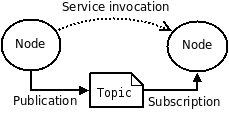
\includegraphics[width=\linewidth]{pictures/ROS_basic_concepts.png}
	\caption{Kommunikation zwischen Nodes}
\end{figure}

Die ROS-Software ist in sogenannten Nodes organisiert, welche die eigentlichen Berechnungen durchf\"uhren. Der ROS-Master hilft den Nodes sich zu finden und eine Verbindung aufzubauen. Die Kommunikation zwischen den Nodes erfolgt dann direkt untereinander über ein ROS spezifisches Protokoll dass auf TCP/IP aufsetzt. Nodes k\"onnen auf Topics ver\"offentlichen und diese abonnieren. \cite{rosConcepts}

Durch die Nodes k\"onnen Funktionalit\"aten wie Planung, Pfadverfolgung, Sensorik, etc getrennt werden. Au{\ss}erdem k\"onnen so einfach Nodes von anderen Leuten genutzt werden. Dies erm\"oglicht es in kurzer Zeit eine Plattform zum Testen der Algorithmen aufzubauen, und ohne gro{\ss}en Aufwand Algorithmen durch Nodes zu implementieren. ROS-Nodes k\"onnen in C++ oder Python geschrieben werden.
\subsection{Hardware}

Die benutzen Roboter haben and der Front einen SICK LMS100 Laserscanner auf einer Höhe von etwa 35 cm motiert. Dieser hat einen Arbeitsbereich von 270° und eine Reichweite von 20 Metern. 

Etwas zu den Motoren schreiben 

\begin{figure}[h]
	\centering
	{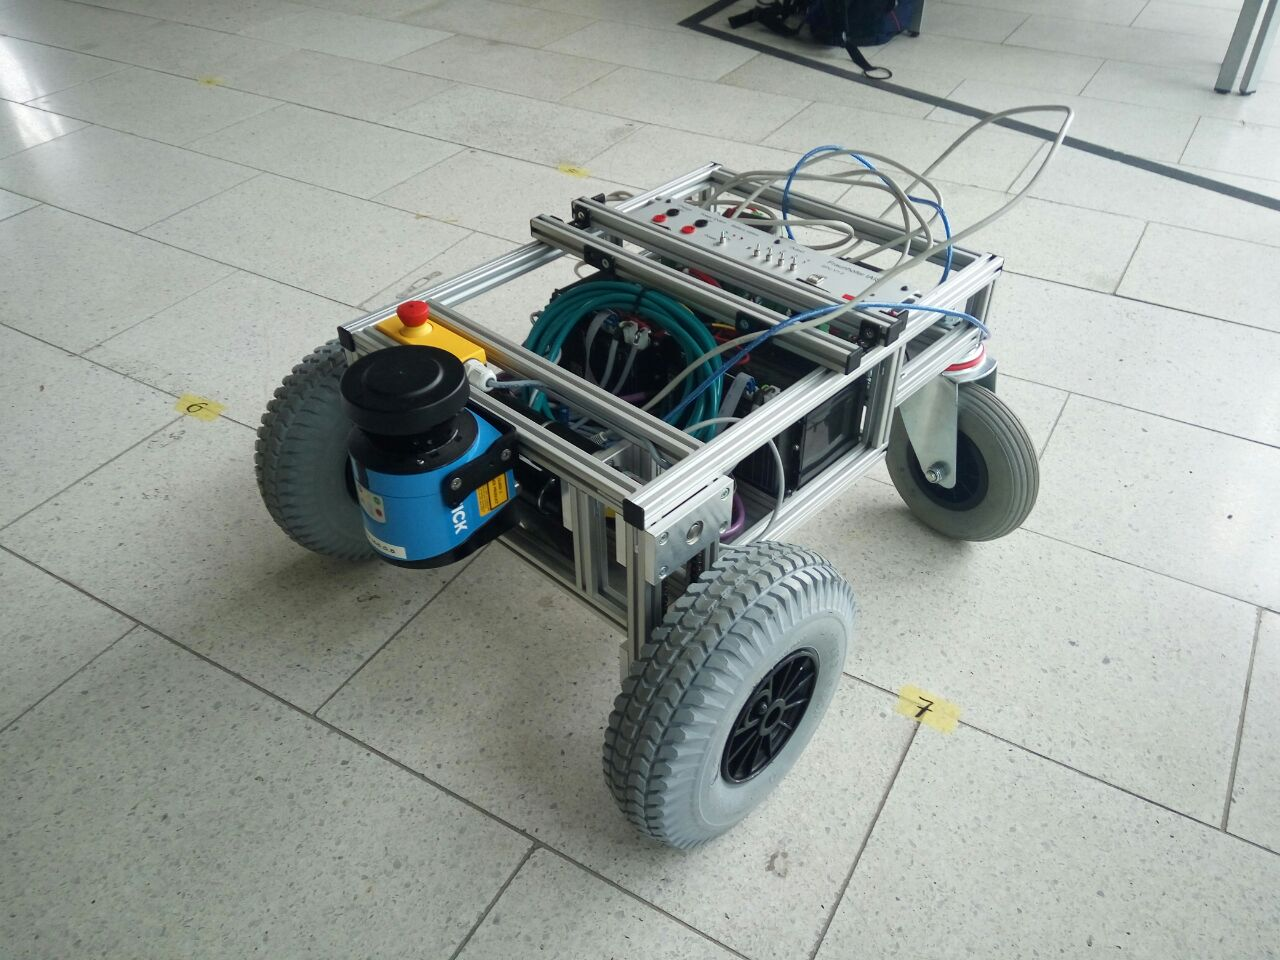
\includegraphics[trim= 2cm 2cm 2cm 2cm, clip=true,width=\linewidth]{pictures/robot.jpg}}
	\caption{Einer der verwendeten Roboter}
\end{figure}


\subsection{Genutzte Nodes}
{
	
	
	\begin{figure*}[h]
		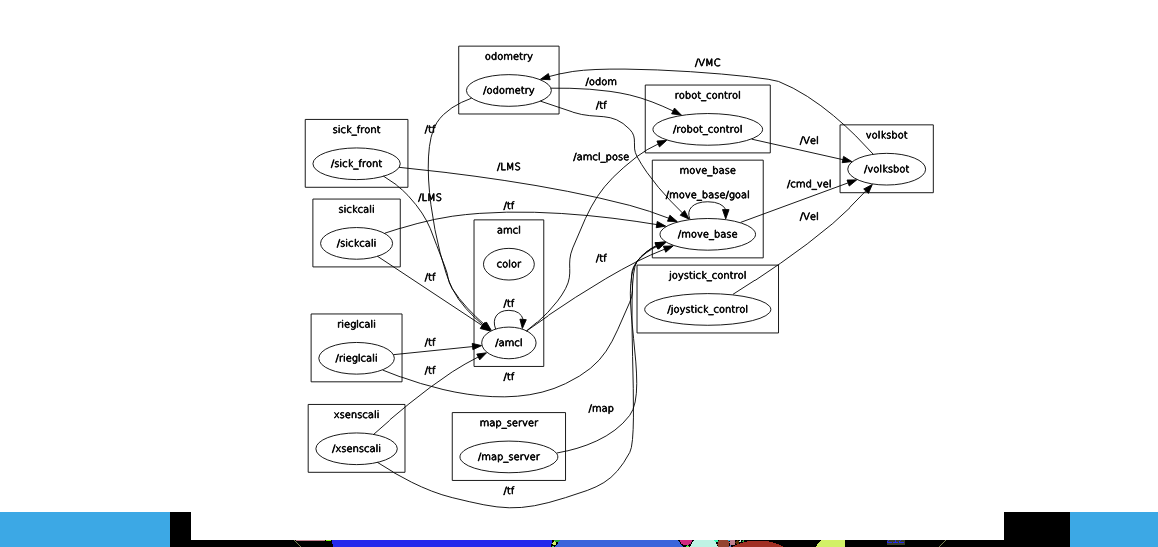
\includegraphics[trim=9cm 1cm 7cm 1cm , clip= true,width=\textwidth]{pictures/node_graph.png}
		\caption{Vernetzung der \textit{Nodes} im Testaufbau}
	\end{figure*}
	
	
	
	 Die Posedaten publiziert die Odometrie an das ROS Paket gmapping.	
	
	
} 

\section{Test der Algorithmen} 
\subsection{Odometrie und AMCL im Vergleich}


Auf kurzen Distanzen liefert die Odometrie sehr genaue Ergebnisse. Mit wachsender Entfernung nehmen auch Fehler durch unterschiedliche Dr\"ucke in den Reifen oder eine verst\"arkte Reibung auf anderem Gel\"ande zu. Weitere Fehlerquelle sind h\"oheren Geschwindigkeiten und engeren Kurven, dort neigen die R\"ader zum Durchdrehen und Wegrutschen. Um das zu zeigen wird der Roboter \"ahnliche Pfade in langsamer und schneller Geschwindigkeit abfahren. 	

Es kann passieren dass AMCL die Anzahl der Partikel so weit verringert das der Zustandsraum nur unzureichend abgedeckt wird. Stimmen die wenigen Hypothesen dann nicht mit der Realität überein verteilt er die Partikel überall hat eine zu geringe Abdeckung des Zustandsraums und schafft es nicht mehr sich zu lokalisieren.

Bild eifügen AMCL verkackt.

Probleme oder eine l\"angere Lokalisierungsdauer treten auch auf, wenn eine Umgebung keine markanten Anhangspunkte liefert, ein kreisf\"ormiger Raum mit glatten W\"anden zum Beispiel. 

Um die Lokalisation durch AMCL und Odometrie miteinander zu vergleichen f\"ahrt der Roboter einen "Acht"-f\"ormigen Pfad ab. Die Steuerung erfolgt manuell \"uber eine Joystick und wird zweimal in verschiedenen Geschwindigkeiten durchgef\"uhrt. Ein Problem entsteht am Anfang, da AMCL nur korrekt arbeitet, wenn die Startpose vorher durch den Benutzer auf den Punkt genau gesch\"atzt wird oder durch Bewegung des Roboters spezifiziert wird. Durch die Bewegung verliert aber die Odometrie an Genauigkeit und startet nicht mehr im Ursprung (0/0). Um Genauigkeit zu garantieren, wird ein Algorithmus verwendet, der die Koordinatensysteme nach der Kalibrierung transformiert.

\begin{figure}[h]
	\centering
	\subcaptionbox{Mit einer Geschwindigkeit $\leq$ 0.8m/s}{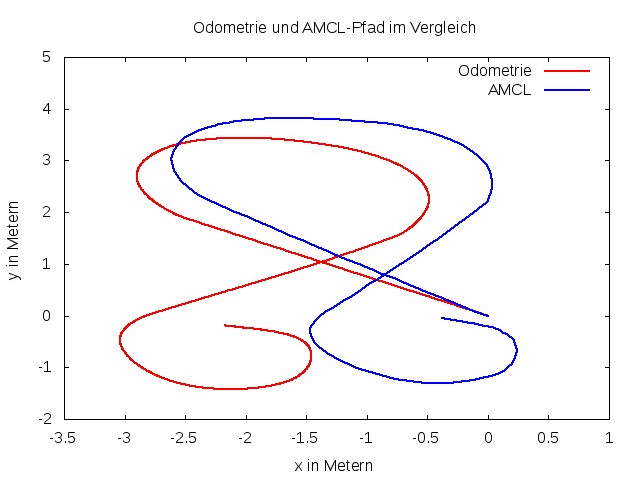
\includegraphics[width=\linewidth]{pictures/odo_amcl_comparision_slow.jpg}}\par\medskip
	\caption{ Odometrie und AMCL im Vergleich. }
\end{figure}




Im Experiment startet der Roboter im Ursprung und bereits zu Beginn kennzeichnet sich ab, dass der Odometriepfad fehlerhaft ist. Bis der Roboter wieder an der Startpose ist, summieren sich die Fehler auf und die Zielpose weicht bis zu 2 m von der Startpose ab. Der AMCL Pfad dagegen, kehrt bis auf wenige Zentimeter zur Startpose zur\"uck. Zus\"atzlich muss in diesem Versuch die menschliche Ungenauigkeit, wie ungenaues Augenma{\ss}, beachtet werden. Aus dem Vergleich ist ersichtlich, dass der Fehler bei AMCL auch in der Distanz, also bei langen Pfaden, nicht gr\"o{\ss}er ist, w\"ahrend bei der Odometrie bei langer Laufzeit die Qualit\"at stetig abnimmt.


Nachteil AMCL: benötigt Karte, Pfad kann nicht in unbekannter Umgebung abgefahren werden

Vorteil: Odometrie ist h\"aufiger und schneller verf\"ugbar da der Rechenaufwand geringer ist. 






\subsection{Test von Gmapping}
{
	Das Untergeschoss des Informatikinstituts W\"urzburg ist mit einem Frauenhofer-Roboter, der mit einem Sick LMS100 Laserscanner ausgestattet ist, in einer 2D-Karte kartiert.  Um diese Karte korrekt aufzunehmen, werden nur so und soviel Partikel ben\"otigt. Die Aufnahme ist bis auf einen 1 cm genau und zeigt keine signifikanten Fehler. Bewegte Objekte wie Menschen werden erkannt und nicht in der Karte verzeichnet. Dagegen sorgt helles Licht, das durch die Fensterfronten scheint f\"ur eine Ungenauigkeit und kann nicht als klare Begrenzung festgestellt werden. F\"ur klare Linie wie W\"ande ist es wichtig, das Gel\"ande mit einem Geschwindgkeitslimit von 2 km/s (halbe Schrittgeschwindigkeit) abzufahren. 
	
	\begin{figure}[h]
		\centering
		\subcaptionbox{fehlerhafte Karte}{
			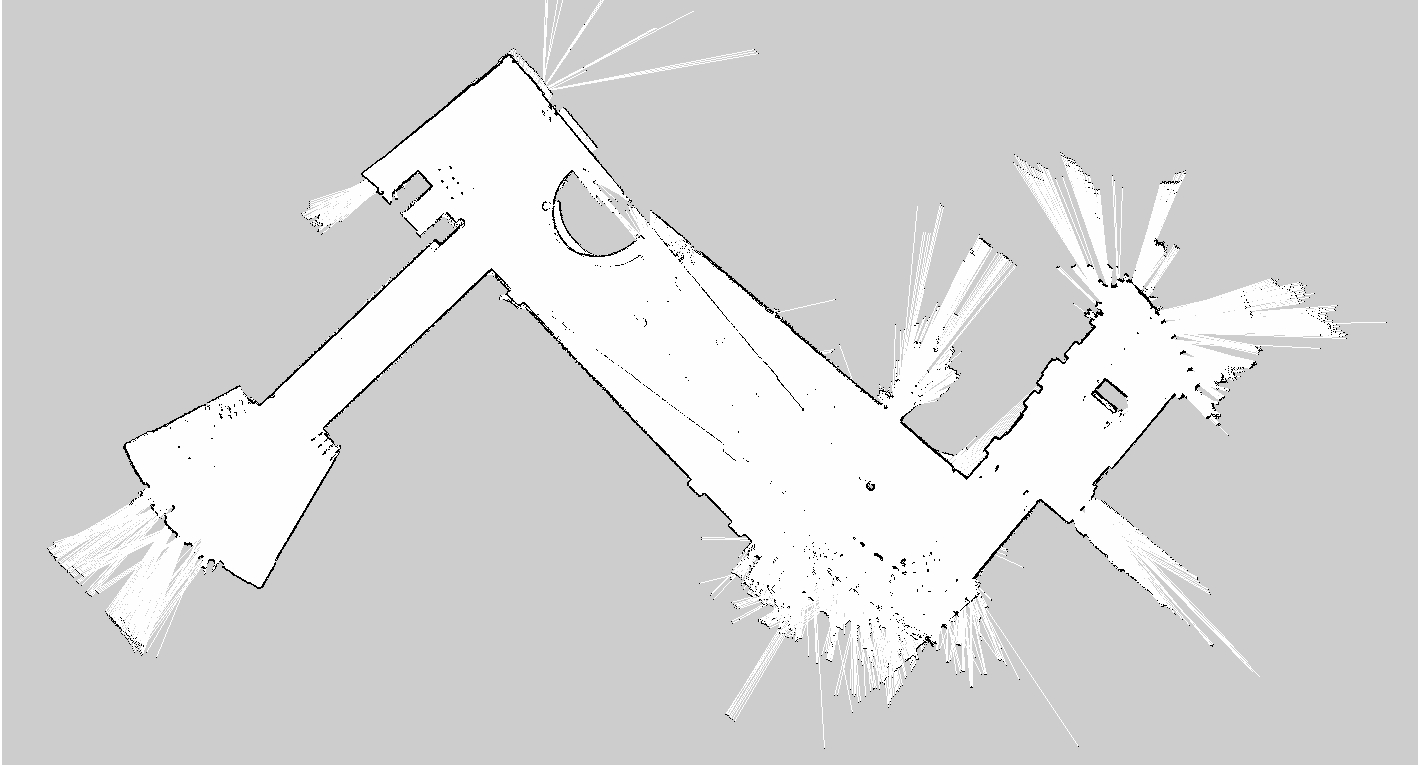
\includegraphics[width=0.45\textwidth]{pictures/firstMap.jpeg}}
		\subcaptionbox{korrekte Karte}{
			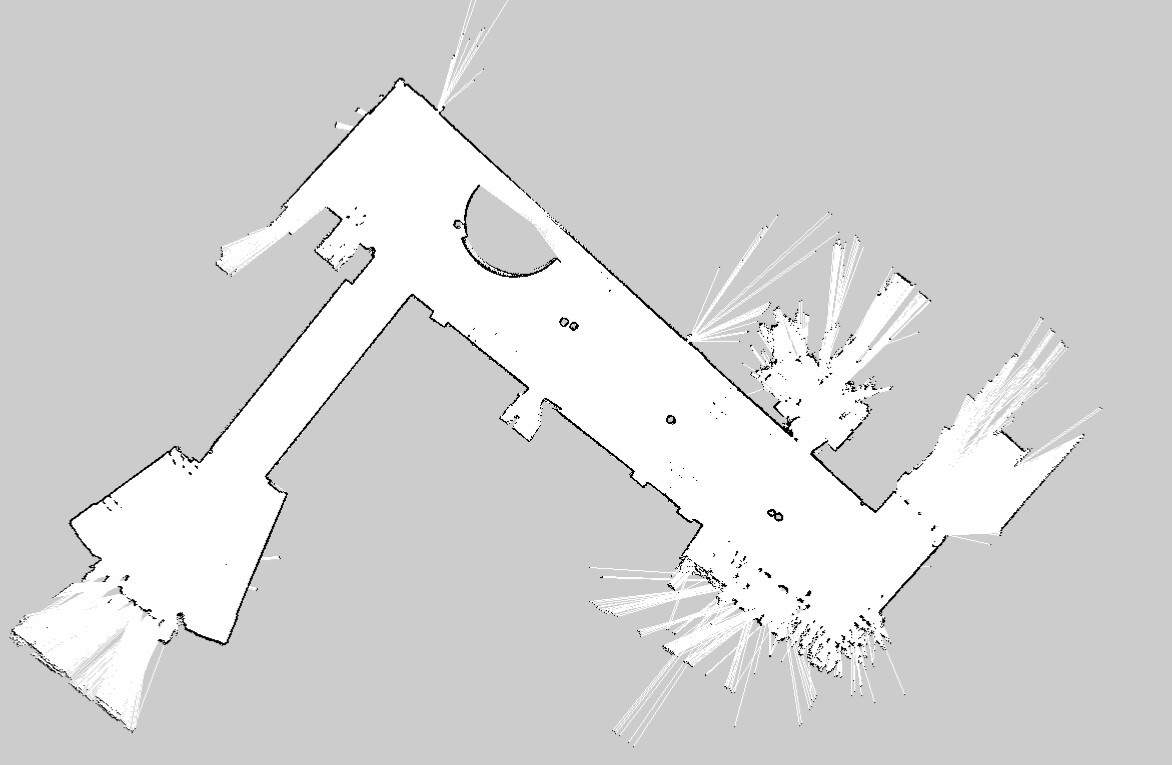
\includegraphics[width=0.45\textwidth]{pictures/correctMap.JPG}}
		\caption{Karten aufgezeichnet mit Gmapping}
	\end{figure}
	
	
	Deutliche Unterschiede sind in den Karten von Figure 4 zu erkennen. Bild (a) zeigt eine Karte, die im ersten Versuch aufgenommen ist und aus Unwissenheit mit zu hoher Geschwindigkeit und nicht oft genug abgefahren ist. Im Vergleich dazu ist die Karte (b) durch langsameres und stetigeres Abfahren detailgetreuer und hat klare Linien.
	
	
	eigene Karte einfügen. AMCL erwähnen.	
}




\subsection{Test und Implementierung von \texttt{gio\_path} auf einem realen Roboter}
Zun\"achst wird die Pfadverfolgung simuliert. Der Robotersimulator wird in ROS-Nodes organisiert und soll vorgebene Pfaddateien abfahren.
\\
\\
Um den \texttt{gio\_path} Algorithmus auf einem realen Roboter zu testen, wird eine ROS-Node verwendet. Diese benutzt  \texttt{gio\_path} um einen realen Roboter zu steuern.
\\


\begin{algorithm}
	
	pathDone $\leftarrow$ false\;
	rightSpeed $\leftarrow$ 0.0\;
	leftSpeed $\leftarrow$ 0.0\;
	controller.setPath(pathFile)\;
	\While{!pathDone}{
		controller.setPose(currentPose)\;
		pathDone = controller.getNextState(leftSpeed, rightSpeed)\;
		publishToMotors(leftSpeed, rightSpeed);
	}
\caption{Giovanni Controller Implementation}
\end{algorithm}

\begin{figure}[h]
	\centering
	\subcaptionbox{niedrige Geschwindigkeit 0,714m/s}{
		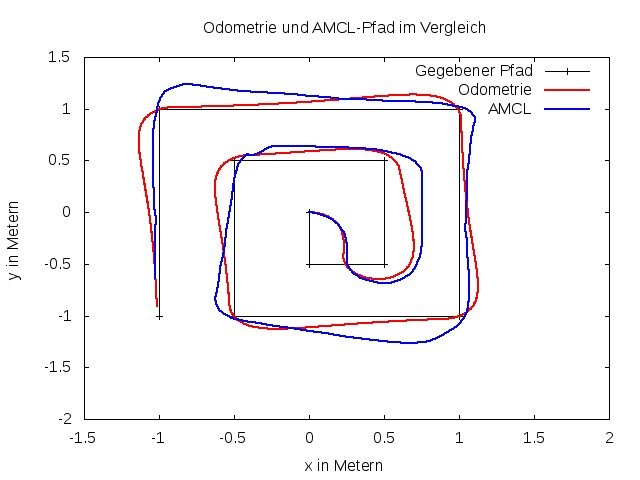
\includegraphics[width=0.45\textwidth]{pictures/path_odometry_slow.jpg}}
	\subcaptionbox{erh\"ohte Geschwindigkeit  3.2 m/s}{
		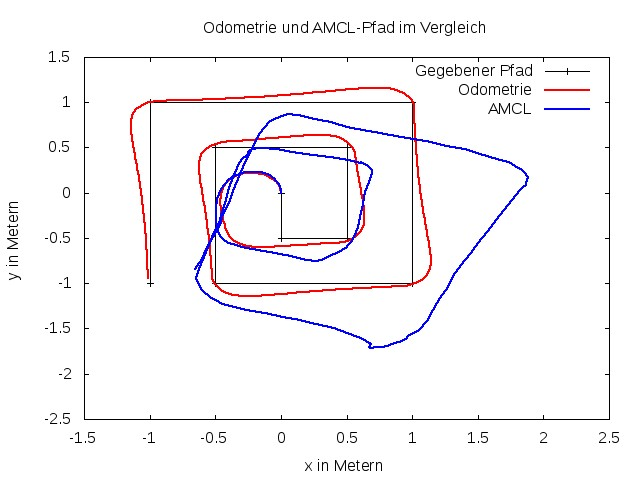
\includegraphics[width=0.45\textwidth]{pictures/path_odometry_fast.jpg}}
	\caption{Pfadverfolgung mit Odometrie}
\end{figure}


\begin{figure}[h]
	\centering
	\subcaptionbox{niedrige Geschwindigkeit 0,714m/s}{
		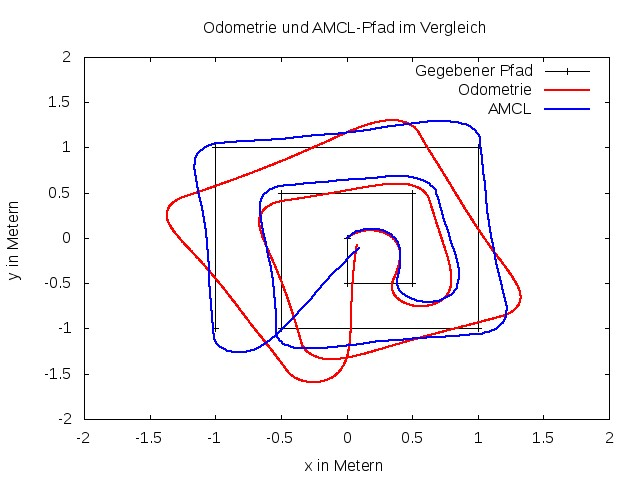
\includegraphics[width=0.45\textwidth]{pictures/path_amcl_slow.jpg}}
	\subcaptionbox{erh\"ohte Geschwindigkeit  3.2 m/s}{
		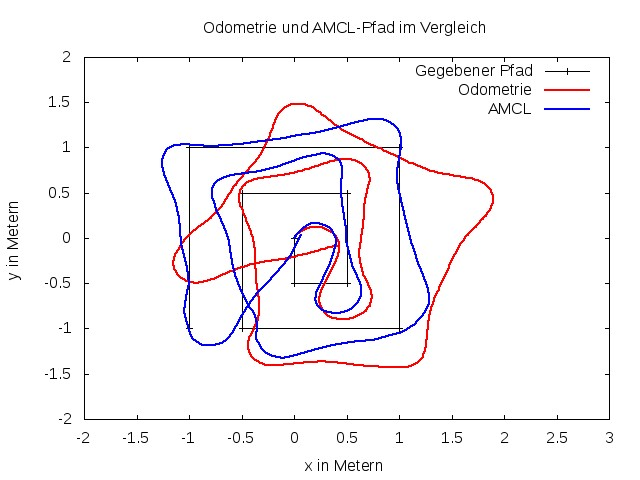
\includegraphics[width=0.45\textwidth]{pictures/path_amcl_fast.jpg}}
	\caption{Pfadverfolgung mit AMCL}
\end{figure}


Die Autoren entscheiden sich als Testpfad eine Spirale zu nutzen. Die Datei enth\"alt Punkte in spiralf\"ormiger, eckiger Anordnung. In dem Vergleich wird der Pfad zweimal abgefahren, einmal in niedriger und einmal hoher Geschwindigkeit. Zu Beobachten ist, dass AMCL bei geringer Geschwindigkeit exakt arbeitet und die Punkte nur auf wenige Zentimeter verfehlt. Bei erh\"oter Geschwindigkeit ist eine Spirale nicht mehr zu erkennen. Die Odometrie zeichnet in beiden F\"allen eine korrekte Spirale auf. Der Grund ist, dass Odometrie unabh\"angig der Umgebung, also ohne Karte, arbeitet und trotz optisch fehlerhaften Pfad die Punkte korrekt skizziert.


Geschwindigkeit langsam: 20  0,714m/s  5cm Genauigkeit
				schnell: 90	 3.2 m/s   20cm 
				
			
				
				 


\section{Zusammenfassung und Ausblick}

Dieses Paper pr\"asentiert den Vergleich zwischen AMCL und Odometrie. Mit einem mobilen Frauenhofer-Roboter wird mittels gMapping eine 2D-Karte erstellt. Die Karte dient dem Roboter sich mit AMCL orientieren, in dem Sensordaten mit Wahrscheinlichkeitsvariablen der Karte verglichen werden. In verschiedenen Vorg\"angen f\"ahrt der Roboter selbst\"andig mittels Pfadverfolgung eine gegebene Punktewolke ab. Die angegebene Punkte werden pr\"azise abgefahren, je dichter der Pfad in Punkten ausgedr\"uckt ist, desto genauer wird der Pfad verfolgt. 
\\
\\
Lokalisierungsschwierigkeiten zeigen sich in bei lautem Rauschen, zum Beispiel in Computerr\"aumen oder in R\"aumen ohne markante Anhaltspunkte. Bewegte Hindernisse wie Menschen stellen bei der Kartierung keine Probleme dar und werden nicht in der Darstellung ber\"ucksichtigt. 
\\
\\
Da Odometrie unabh\"angig von seiner Umgebung einen Pfad verfolgt, ist AMCL 
Es zeigt sich das Odometrie schlechter als AMCL ist.

Als weiteres ist geplant...


\section{Danksagung}
Die Autoren danken Angel f\"ur die Unterst\"utzung und Hilfe bei verschiedenen Problemen mit dem Roboter und \textit{Robot Operating System}.

\newpage
{%\small                   % use small if you need it
	\bibliographystyle{plain}
	\bibliography{paper.bib}       % use a bib-file paper.bib to collect

\end{document}








